The \ac{TCA} implementation for the \ac{CMR} is one that heavily utilizes geometry and a rigid-body model assumption, while also placing an emphasis on relying on minimal assumptions/data about the environment and avoiding computationally complex calculations on input data from sensors, cameras, etc. There were various reasons as to why some of these assumptions/choices were made and why the agreed upon implementation was deemed the best choice for the given scenario \cite{tractl}, which is expanded on later in the document. Figure~\ref{traction_control:introduction:scarecrow} shows a testbed version of the \ac{CMR}.

\begin{figure}[htbp]
	\centering
	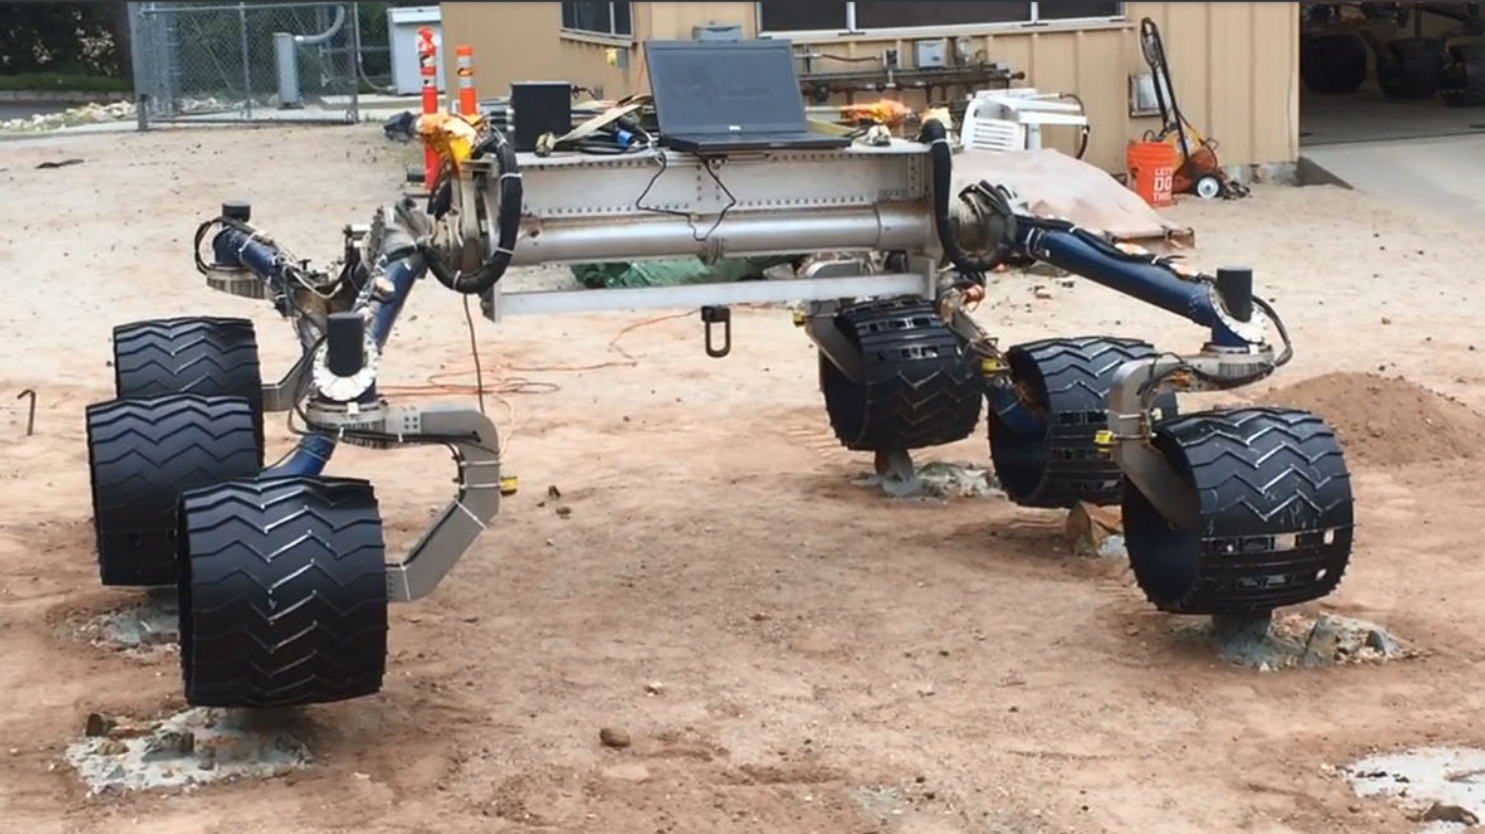
\includegraphics[width=.9\textwidth]{sections/introduction/images/scarecrow_testbed.png}
	\caption{The Scarecrow Testbed Rover, a Rover Kinematically Similar to the \acl{CMR} \cite{tractl}}
	\label{traction_control:introduction:scarecrow}
\end{figure}

It is important to note that the need for this \ac{TCA} was not discovered until after the flight system was actively engaging in its mission on the Martian surface, while ground control was observing telemetry of its use. Therefore, it was impossible to make any physical modifications to the \ac{CMR}, only software could be remotely flashed to it. \\

However, there are still ramifications to having this additional routine run on the \ac{CMR}. The limited computational resources available to do so must be considered carefully, so as to not interfere with existing processes being ran, and the implementation chosen has to have enough resources to perform the task it needs to as well. The team responsible for solving the problem at hand clarified some of these issues and how it restricted their choices for strategies to solve the problem. For example, the rover ``does not include force or torque sensors on the mobility subsystem, nor can it measure slip with high enough frequency to be able to react to it.'' \cite{tractl} Some of the characteristics and assumptions of the \ac{CMR} and its \ac{TCA} implementation are discussed in Section~\ref{traction_control:discussion:prereqs}. \\

This algorithm was chosen to study because of the advantages it has over other possible implementations, some of which were considered by the team that came up with this original \ac{TCA} solution. Aspects of the \ac{SRR} were being modeled for another course, so consideration was taken in applying the concepts of this solution and attempting to utilize them on this kinematically different vehicle, an image of which can be seen in Figure~\ref{traction_control:introduction:srr}. A 3D rendering of a model similar to the \ac{SRR} was generated, as well as a simulation suite that's able to interact with it, including an implementation of the algorithm. At the time of finishing this report, the simulation suite is still in its early stages and has limited functionality.

\begin{figure}[htbp]
	\centering
	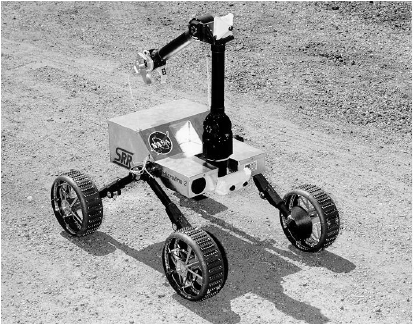
\includegraphics[width=.9\textwidth]{sections/introduction/images/srr.png}
	\caption{The \acl{SRR} \cite{srr}}
	\label{traction_control:introduction:srr}
\end{figure}
